\section{Processes and Concurrency}

\subsection{Description}
% GOAL V02 • You can explain tasks/processes, process states, context switches and scheduling/dispatching.
% GOAL V02 • You can explain the principles of multitasking and concurrency.
% GOAL V02 • You can understand and utilize a selected RTOS, the FreeRTOS, to create and manage tasks.

Every process possesses its own context.
That consists of:
\begin{itemize}
    \item \textbf{Memory context:} Memory used by the process (program code, stack)
    \item \textbf{Hardware context:} Registers (PC, SP, PSR)
    \item \textbf{System context:} OS intern management data of the process (called \textbf{TCB})
\end{itemize}

% TODO : Maybe add Task Control Block (TCB)

\subsection{Process vs Thread model}
% GOAL V02 • multitasking and concurrency (FreeRTOS tasks)

In FreeRTOS, a thread is called a task.
In this context it can be used interchangeably.

When allowing multiple threads, they can be changed with each sysTick.
However, the context has to be saved.
To minimize this overhead, it is important to minimize task switches when possible.

\subsubsection{Steps for a context switch}
% GOAL V02 • tasks/processes, states, context switch, scheduling, multitasking, FreeRTOS

\begin{enumerate}
    \item Save the context of the interrupted process 1
    \item Change the status of process 1 to \emph{Ready} or \emph{Waiting} (depending on the reason for the interruption)
    \item Selection of the process 2 to be activated by the scheduler
    \item Change the status of process 2 from \emph{Ready} to \emph{running}
    \item Restoring the (saved) context of process 2 by loading the processor registers
\end{enumerate}

\begin{center}
    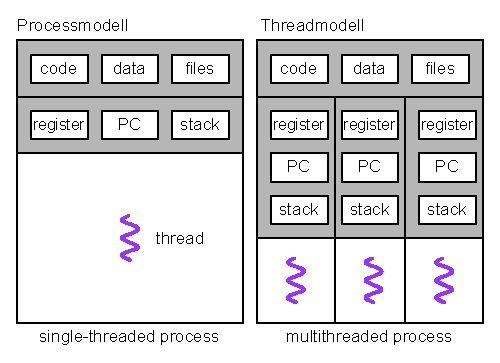
\includegraphics[width=0.8\columnwidth]{images/PDF/process_model.pdf}
\end{center}


\subsection{Process states}
% GOAL V02 • process states

\begin{itemize}
    \item \textbf{Inactive:} ``Formal'' state for processes that do not yet or no longer exist in the system.
    \item \textbf{Ready:} The process is waiting for the allocation of a processor (no further wait conditions apply). 
    If multiple processes are in the Ready state, the operating system decides, based on its scheduling policy, 
    which one may switch to the Running state.
    \item \textbf{Running:} The process has been allocated a processor, and it is running. 
    In a single-processor system, a maximum of one process can be in this state.
    \item \textbf{Waiting:} The process is waiting for the fulfillment of at least one wait condition.
\end{itemize}

\subsubsection{Transitions}

A state transition may happen for the following reason:

\begin{tabular}{lcll}
    \textbf{Inactive}   & $\Rightarrow$ & \textbf{Ready}    & A process is generated \\
    \textbf{Ready}      & $\Rightarrow$ & \textbf{Running}  & The process gets execution time\\
    \textbf{Running}    & $\Rightarrow$ & \textbf{Ready}    & A different process gets priority\\
    \textbf{Running}    & $\Rightarrow$ & \textbf{Waiting}  & A waiting condition occurs\\
    \textbf{Waiting}    & $\Rightarrow$ & \textbf{Ready}    & All waiting conditions got fulfilled\\
    \textbf{Running}    & $\Rightarrow$ & \textbf{Inactive} & The process is finished and stops\\
    \textbf{Waiting}    & $\Rightarrow$ & \textbf{Inactive} & The process is aborted (by OS or other process)\\
    \textbf{Ready}      & $\Rightarrow$ & \textbf{Inactive} & The process is aborted (by OS or other process)
\end{tabular}

\begin{center}
    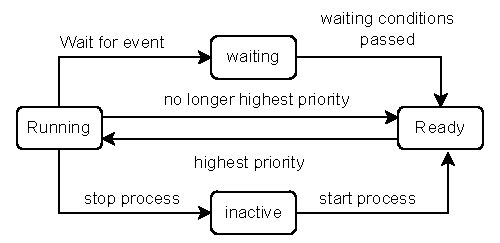
\includegraphics[width=0.8\columnwidth]{images/PDF/transitions.pdf}
\end{center}

\subsection{Scheduling}
% GOAL V02 • scheduling policies, scheduling problem, execution time, preemption
% GOAL Lab 02 • You can understand the basics of a scheduler and a dispatcher, as well as how they relate to each other.

Scheduling policies are different strategies to maximize some metrics (and improve system performance in):

\begin{itemize}
    \item \textbf{CPU utilization:}CPU utilization should be optimized.
        The goal is 100\% CPU utilization; otherwise, 40\%\-90\% is typical.
    \item \textbf{Throughput:} Number of tasks completed per unit of time. 
        This is a measure of system utilization.
    \item \textbf{Fairness:} No task should be given preferential treatment. 
        On average, every user should receive the same share of CPU time.
    \item \textbf{Turnaround time:} The time span from the start to the end of the task.
        This includes all times for queues, execution (processing time), and input and output.
    \item \textbf{Waiting time:} The scheduler cannot influence execution time, only the waiting times in the waiting and ready lists. 
        The goal is to minimize these waiting times.
    \item \textbf{Response time:} Users find it particularly frustrating when a system response is delayed (high latency). 
        The goal is to minimize the response time between input and the resulting response.
\end{itemize}

% TODO maybe add time definition (V02 slide 42)

\subsubsection{Scheduling problem}

The correct and effective scheduling of tasks is a difficult problem to solve and involves the following design criteria

\begin{itemize}
    \item Time restriction (Deadlines): hard vs.~soft (vs.~no deadlines)
    \item Task-Periodicity: periodic vs.~aperiodic (vs.~sporadic)
    \item Cooperation: preemptive vs.~non-preemptive
    \item Design-/Run-Time: static vs.~dynamic
    \item Task-dependencies: dependent vs.~independent
\end{itemize}

\resizebox{\columnwidth}{!}{%
\begin{tikzpicture}[
  font=\sffamily,
  >=Latex,
  edge/.style={->, line width=0.6pt},
  level 1/.style={sibling distance=30mm, level distance=10mm},
  level 2/.style={sibling distance=70mm,  level distance=10mm},
  level 3/.style={sibling distance=38mm,  level distance=10mm},
  level 4/.style={sibling distance=18mm,  level distance=10mm},
  every node/.style={align=center},
]

\node (root) {real--time scheduling}
  child[edge] { node {hard deadlines}
    child[edge] { node {periodic}
      child[edge] { node {preemptive}
        child[edge] { node {static} }
        child[edge] { node {dynamic} }
      }
      child[edge] { node {non--preemptive}
        child[edge] { node {static} }
        child[edge] { node {dynamic} }
      }
    }
    child[edge] { node {aperiodic}
      child[edge] { node {preemptive}
        child[edge] { node {static} }
        child[edge] { node {dynamic} }
      }
      child[edge] { node {non--preemptive}
        child[edge] { node {static} }
        child[edge] { node {dynamic} }
      }
    }
  }
  child[edge] {node {soft deadlines}};
\end{tikzpicture}
}

\subsubsection{\textit{Firmness} Of time systems}
\begin{itemize}
\item \textbf{Hard}: Missing deadline may cause catastrophic consequences on the system.
\item \textbf{Firm}: Getting results after its deadline is useless for the system, but does not cause any damage.
\item \textbf{Soft}: Producing the results after its deadline has some utility for the system, although causing a performance degradation.
\end{itemize}

\subsubsection{Execution time}
\label{sec:execution_time}

The execution time of a task can be calculated by
\begin{equation*}
    \boxed{\text{Time} = 
    \frac{\text{Seconds}}{\text{Program}} = 
    \frac{\#\text{Instructions}}{\text{Program}} \frac{\text{Clock cycles}}{\text{Instruction}} \frac{\text{Seconds}}{\text{Clock cycle}}}
\end{equation*}

\subsubsection{Preemption}{verdrängung}

When pursuing a non-preemptive scheduling policy, the tasks are always run to completion.
Only when the tasks itself yields, can a context switch occur.
This reduces overhead of context switches, but it also increases response time.

The following example shows 3 concurrent, cyclical tasks in a preemptive and non-preemptive situation.
The tasks' priority is \( \text{A} > \text{B} > \text{C}\).
A occurs every \qty{6}{\second}, B every \qty{9}{\second} and C every \qty{3}{\second}.

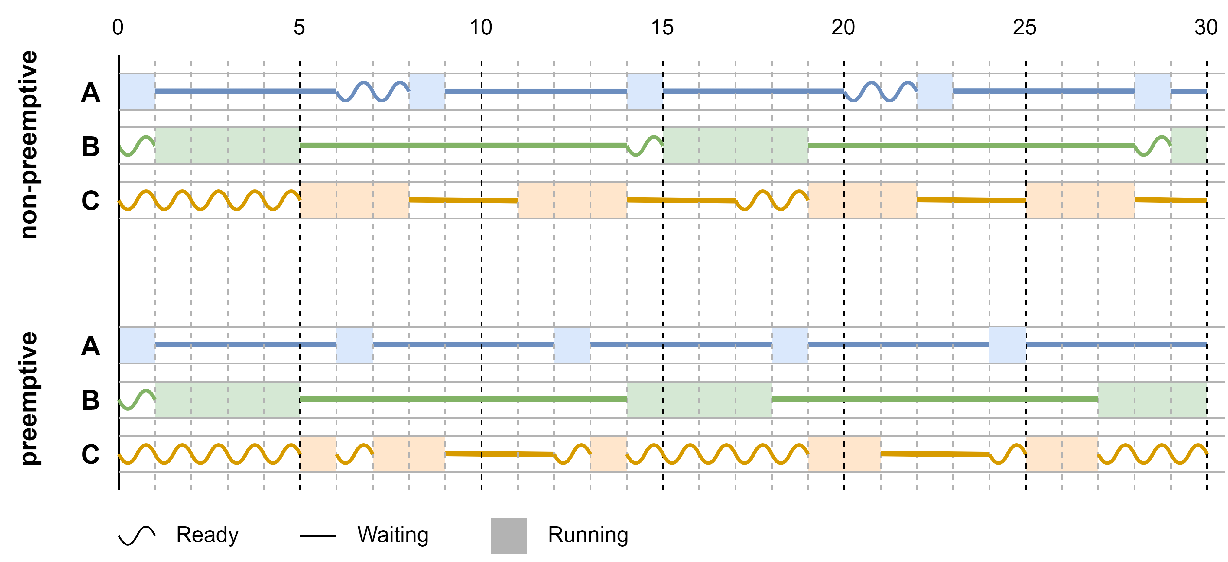
\includegraphics[width=\columnwidth]{images/preemptive_vs_non.png}

With preemptive scheduling, more context switches occur, but higher priority tasks are always executed on time.

All modern OS's use preemptive scheduling, this however has the consequence that task execution is less predictive.
In general the \emph{safe bet} is to use non-preemptive scheduling.

\textbf{Scheduling of FreeRTOS}

The scheduling of FreeRTOS executes tasks with the highest priority and then shares CPU time between similar priorities (so-called round-robin).
% TODO maybe add more scheduling stuff

\subsection{Inter-Process communication}
% GOAL V03/V04/L04/L05 • IPC, mutex, semaphore, queues, deadlocks, priority inversion

Interprocess communication is done via mutexes and semaphores.
They can be taken (p~operation) or released (v~operation).
Typically the semaphore (binary) is taken before entering a critical section and released after

\subsubsection{Mutex}
    % GOAL L04 • You understand the difference between a semaphore and a mutex.
    A mutex is \textbf{a locking mechanism} used to protect a shared resource.
    \begin{itemize}
        \item Must be taken and released by the same task.
        \item Has an ``owner''.
        \item Is typically initialized in the unlocked state (i.e., token is available).
        \item boolean valued
    \end{itemize}

\subsubsection{Semaphore change in ISR}
\label{Mutex_From_ISR}
When a semaphore is given, a previously blocked task might become unblocked.
To remove additional overhead, the current executed task can directly be set to the now ready task without waiting for an additional systick:
\begin{lstlisting}
extern "C" void button_pressed_callback_bin_sem(){
	portBASE_TYPE higher_task_unblocked = pdFALSE;
	buttonPressedSemHandle->give_ISR(higher_task_unblocked);
	portYIELD_FROM_ISR( higher_task_unblocked );
}
\end{lstlisting}

\subsubsection{Semaphore}
    % GOAL L04 • You understand the difference between a semaphore and a mutex.
    A semaphore is \textbf{a signaling mechanism} used to notify a waiting task that it can proceed.
    \begin{itemize}
        \item Can be manipulated from different tasks; any can execute \texttt{give} and \texttt{take}.
        \item Has no ``owner''.
        \item At initialization it is typically empty (i.e., no available token).
        \item Integer valued
    \end{itemize}

\subsubsection{Semaphore vs. Mutex}
\begin{tabular}{p{0.45\columnwidth} p{0.45\columnwidth}}
\hline
\textbf{Semaphore (signaling mechanism)} & \textbf{Mutex (locking mechanism)} \\
\hline
Binary: synchronization, mutual exclusion & Binary semaphore \emph{with} ownership \\
Counting: resource management, event counting & \emph{and} priority-inheritance mechanism \\
Any task/ISR may give or take & Only the owning task releases \\
\hline
\end{tabular}
Use a mutex for higher safety when guarding a shared resource (ownership, recursive locking, task-deletion safety, priority-inversion avoidance).

\subsubsection{Synchronize tasks using a Semaphore}
% GOAL L04 • You can synchronize multiple tasks with semaphores.
% GOAL V04 • You can implement IPC concepts with these RTOS objects in FreeRTOS.

Using semaphores, tasks can be synchronized by releasing the semaphore when done and waiting for the other to be released.

\begin{minipage}{0.49\columnwidth}
\textbf{correct}

\begin{minipage}{0.49\columnwidth}
Task a
\begin{lstlisting}
// statements
aMutex.give()
bMutex.take()
// synchronized 
\end{lstlisting}
\end{minipage}
\begin{minipage}{0.49\columnwidth}
Task b
\begin{lstlisting}
// statements
bMutex.give()
aMutex.take()
// synchronized
\end{lstlisting}
\end{minipage}
\end{minipage}
\begin{minipage}{0.49\columnwidth}
\textbf{Incorrect (deadlock)}

\begin{minipage}{0.49\columnwidth}
Task a
\begin{lstlisting}
// statements
bMutex.take()
aMutex.give()
// never reached
\end{lstlisting}
\end{minipage}
\begin{minipage}{0.49\columnwidth}
Task b
\begin{lstlisting}
// statements
aMutex.take()
bMutex.give()
// never reached
\end{lstlisting}
\end{minipage}
\end{minipage}

\subsection{Priority inversion}
% GOAL V04 • You can explain priority inversion and how it can be dealt with via resource access protocols.
Under \emph{priority-based preemptive} scheduling, a low-priority task holding a resource blocks a higher-priority task (HPT).
A resource-access protocol can prevent this.
\subsubsection{Resource-access protocols}
\begin{outline}
  \1 \textbf{Priority Inheritance (PIP):} raise the LPT's priority to the HPT's while it holds the resource; bounds inversion (promotion is \emph{transitive} along the blocking chain). Does \emph{not} prevent deadlock from bad lock ordering.
  \1 \textbf{Priority Ceiling (PCP):} the \emph{ceiling} of a resource is the highest priority of any task that may request it. A task inherits the ceiling on acquisition (or may only enter if its priority exceeds the system ceiling); on release its priority drops to the highest ceiling still held. \textbf{Prevents deadlock} by ordering resources.
\end{outline}

% If a lower priority task acquires a mutex that a higher priority task needs, the lower priority task is \say{upgraded} to the higher priority.
% That way the higher priority task does stay blocked shorter, or it even circumvents a deadlock.


\subsection{Message Queues}
% GOAL V04 • You can explain how message queues and message or stream buffers/pipes work and how they are used (best practices).

A \textbf{message queue} is a buffer-like kernel object through which tasks/ISRs exchange messages (with data), \textbf{decoupling} sender and receiver (they need not run simultaneously).
A queue can be \textbf{Empty}, \textbf{Not Empty} or \textbf{Full}. 
Sending to a full queue or receiving from an empty one can \textbf{block} the caller.
\subsubsection{Data vs. pointer}
\begin{ctabular}{p{0.46\linewidth}p{0.46\linewidth}}
\textbf{By value (copy)} & \textbf{By reference (pointer)} \\ \hline
two copies (sender\textrightarrow{}queue\textrightarrow{}receiver); good for \emph{small} messages. & queue holds a pointer to a shared buffer; good for \emph{large} messages. \\
\end{ctabular}

\subsection{Pipes \& Buffers}
\textbf{Pipes} provide \emph{unstructured} byte exchange and synchronization: the reader blocks when empty, the writer when full. A \textbf{select} operation blocks on a condition over one or several pipes. FreeRTOS has no pipes; alternatives: \textbf{queues}, \textbf{stream buffers} (single reader/writer byte stream, e.g.\ ISR\textrightarrow{}task or core-to-core) and \textbf{message buffers} (discrete variable-length messages on top of stream buffers).

\subsection{Locks vs.\ Lock-Free}
Queues are a quasi lock-free instrument: transferring data ownership avoids explicit locks. 
A gatekeeper task with sole ownership of a resource (no locking), or a shared memory pool passed by reference can serve as the sole handler of critical structures.

\subsection{Deadlocks}
A \textbf{deadlock} permanently blocks threads because their resource needs can never be satisfied (possible whenever the RTOS shares resources and a thread may hold several).

\subsubsection{Coffman conditions}
All four must hold for a deadlock:
\begin{ctabular}{ll}
Mutual exclusion & resource used by one task at a time \\
No preemption & freed only by its holder \\
Hold and wait & holds some, waits for more \\
Circular wait & cyclic chain of holders/requesters \\
\end{ctabular}

\subsubsection{Prevention} 
Negate one condition:
\begin{outline}
  \1 \textbf{No preemption:} release held resources if a new request is denied, then re-request all together.
  \1 \textbf{Hold and wait:} request \emph{all} resources at once.
  \1 \textbf{Circular wait:} acquire resources in one global \textbf{ascending order} (\emph{forward strategy}).
\end{outline}
Mutual exclusion is usually not eliminable. 
Assess deadlock risk over \emph{all} processes together, not pairwise.
